\documentclass[12pt]{article}
 \usepackage[german]{babel}
 \usepackage[utf8]{inputenc}
 \usepackage{listings}
  \usepackage{color}
 \usepackage{graphicx}
 \author{Denis Herdt, Almin Causevic}
 \title{ROS auf dem Rapberry Pi}
 \setlength{\parindent}{0pt}                   % Einrueckung 1. Zeile eines Absatzes
 \setlength{\parskip}{5pt plus 2pt minus 1pt}  % Abstand zwischen Absaetzen
 \frenchspacing
 \sloppy
  \lstset{
   basicstyle=\small\ttfamily,
   keywordstyle=\bfseries\ttfamily\color{orange},
   stringstyle=\color{green}\ttfamily,
   commentstyle=\color{middlegray}\ttfamily,
   emph={square}, 
   emphstyle=\color{blue}\texttt,
   emph={[2]root,base},
   emphstyle={[2]\color{black}\texttt},
   showstringspaces=false,
   flexiblecolumns=false,
   tabsize=2,
   frame=tBlR
   numbers=left,
   numberstyle=\tiny,
   numberblanklines=false,
   stepnumber=1,
   numbersep=10pt,
   xleftmargin=15pt
 }
 
 
\begin{document}
%4-20 Seiten
\begin{figure}[h]


\includegraphics[width=4cm]{hs-logo.jpg}
\end{figure}
Fakultät für Elektrotechnik und Informatik

\vspace{3cm}

\begin{center}

{\bf \huge ROS auf dem Raspberry Pi}
\vspace{4cm}

14 November, 2013
\vspace{1cm}

Systemadministration Projekt in Angewandter Informatik \\
von Denis Herdt und Almin Causevic

\end{center}

\pagebreak

\tableofcontents

\pagebreak

\section{Einleitung}
%1-2 Seiten
\subsection{Motivation}

Die Entscheidung für dieses Thema fiel dadurch, dass es zukünftig genutzt werden kann und Soft-/Hardware kombiniert werden.

Im Robotiklabor der Hochschule Weingarten wird außerdem zur Zeit noch umsändlich ein zusätzlicher Laptop zur Steuerung der Roboter verwendet. Ein Beispiel dafür ist der ''Volksbot''. Durch die zusätzliche Last werden Platz, Gewicht und Stom stärker beansprucht. Dieses Problem kann mithilfe des kleinen und leichten Raspberry Pi gelöst werden.

Durch den Einsatz des Software-Frameworks ROS (Robot Operating System) kann ein flexibles Netzwerk von Komponenten realisiert werden, in das der Raspberry eingebunden wird. Dies ist zur Zeit die aktuellste und inovativste Methode Robotersteuerung zu realisieren. ROS wird weltweit eingesetzt und kann auch in Zukunft sehr nützlich sein.

Durch die Kombination mit der Mächtigkeit und Flexibilität von ROS und der gerinen Größe und niedrigen Energieverbrauch des Pi eröffnen sich neue und effiziente Einsatzmöglichkeiten.

Zudem ist dieses Projekt für das Fach Sysadministration sinnvoll, weil mit Linux gearbeitet wird und viel Konfiguration des Betriebssystems vorausgesetzt wird.

%ROS ist zur Zeit die aktuellste und inovativste Methode, ein flexibles Netzwerk von Komponenten für z.B. die Robotersteuerung zu realisieren. Es wird weltweit eingesetzt und kann auch in Zukunft sehr nützlich sein.

%Wir haben uns für dieses Thema entschieden, weil wir mit Hard- und Software arbeiten wollten.

%Wir haben mitbekommen, wie umständlich z.B. der Roboter ''Volksbot'' im Robotiklabor der Hochschule mit einem zusätzlichen, auf dem Roboter platzierten Laptop gesteuert werden muss, der unnötig Platz und Gewicht beansprucht. Deshalb haben wir uns entschlossen, dieses Problem mithilfe des kleinen und leichten Raspberry Pi zu lösen.
%Die Idee stieß auch auf großes Interesse bei den Labormitarbeitern und bringt viel praktischen Nutzen.

%Unser Ziel möchten wir mithilfe des Software-Frameworks ROS (Robot Operating System) realisieren.
%Für ROS haben wir uns entschieden, weil es zur Zeit die aktuellste und inovativste Methode ist, ein flexibles Netzwerk von Komponenten für z.B. die Robotersteuerung zu realisieren. Es wird weltweit eingesetzt und könnte auch in Zukunft sehr nützlich werden.

%Durch die Kombination mit der Mächtigkeit und Flexibilität von ROS und der geringen Größe und dem niedrigen Energieverbrauch des Pi eröffnen sich außerdem neue und effizientere Einsatzmöglichkeiten.

%Sehr gut finden wir auch die Tatsache, dass wir mit Linux arbeiten können und dieses Projekt viel Konfiguration des Betriebssystems voraussetzt, da wir auch gerne mehr Praxiserfahrung mit Linux haben möchten.





%Roboter Lab Anwendung von ROS und Möglichkeit, Roboter zu nutzen

%Interesse der Lab-Crew an Umsetzung ROS mit Raspberry Pi

%Kombination Hard-/Software

%Einarbeitung in Kommunikations Framework ROS

%Mit Hardware in Berührung zu kommen

%Konfiguration mit Linux

%Nodes nun mit Hardware (Pi) realisierbar

\subsection{Zielsetzung}


Unser Hauptziel besteht darin, ROS auf dem Raspberry Pi aufzusetzen und zu nutzen. Dieses Ziel wird wie folgt unterteilt:\\

\begin{itemize}

\item Recherche über Linux Systeme auf dem Raspberry Pi 
\item Passendes Linux System auf Raspberry Pi aufsetzten			
\item Recherche über ROS
\item Geeigneten Roboter wählen (Recherche Verfügbarkeit, Komponenten etc.)
\item Komponenten geschaffen (Wlan Stick, Akkupack, etc.)
\item ROS auf Raspberry Pi aufsetzen
\item Netzwerk zwischen mehreren ROS-Komponenten herstellen
\item Netzwerk mithilfe von Testausgaben überprüfen

\end{itemize}

Mit diesen Zielen ist eine Grundlage für weitere Anwendungen mit ROS auf dem Raspberry geschaffen.\\

{\bf optional}

Da uns am Ende noch genügend Zeit zur Verfügung stand, haben wir folgende Punkte bearbeitet:

\begin{itemize}

\item Steuerungspaket für ''Volksbot'' einbinden
\item Verbesserung der Usability durch Smartphone-Steuerung
\item Optimierung der WLAN-Verbindung am Raspberry
 
\end{itemize}
Bleibt am Ende noch genug Zeit, wird die integriete Kamera des Roboters angesprochen und das Bilde mithilfe des Netzwerkes auf einen externen Bildschirm übertragen.

%Zunächst möchten wir ein passendes, auf Linux basierendes Betriebssystem auswählen und auf dem Raspberry Pi aufsetzen. In diesem Fall haben wir uns für Raspbian entschieden, da es zusätzlich am kopatibelsten zu ROS ist.

%Als nächstes wählen wir einen geeigneten Roboter aus. Die Kriterien dafür erarbeiten wir uns aus einer vorangegangenen ROS-Recherche.

%Im Anschluss setzen wir ROS auf dem Raspberry Pi und mehreren Linux-Rechnern auf und stellen ein WLAN-Netzwerk zwischen den verschiedenen ROS-Komponenten her.
%Dieses Netzwerk wird mithilfe von Testausgaben überprüft.

%Damit ist eine Grundlage für weitere Anwendungen für ROS auf dem Raspberry geschaffen.\\

%{\bf optional}

%Bleibt am Ende noch genug Zeit, kompilieren wir ein Steuerungspaket für den ''Volksbots'' auf dem Raspberry. Zur Verbesserung der Usability integrieren wir ein Smartphone ins ROS-Netzwerk. Die Bewegungsrichtung und -geschwindigkeit des Roboters soll durch das Schwenken des Smartphones bestimmt werden.

%Haben wir damit Erfolg und wiederum genügend Zeit zur Verfügung, sprechen wir die integrierte Kamera des Roboters an und streamen das Bild mithilfe des Netzwerkes auf einen externen Bildschirm.

%Da zukünftige Roboter Ihre Umgebung erkennen und sich sicher im Raum bewegen sollen, sehen wir diese Tests als nützlich an.

%Roboter durch einen Raspberry Pi mithilfe von ROS steuern
%Bild einer Webcam durch ROS auf einen Bildschirm streamen

\subsection{Eigene Leistung}

Das ''neue'' an diesem Projekt bezieht sich
%Unsere Leistung bezieht sich
auf die Ablösung eines Laptops durch den kleineren und leichteren Raspberry Pi als ROS-Komponente am ausgewählten Roboter. Desweiteren möchten wir herausfinden, ob die Leistung des Pi für diese Aufgabe ausreicht.

%anstatt Linux PC wird Pi benutzt

\subsection{Aufbau der Arbeit}

In den Grundlagen werden alle wichtigen Komponenten und Aspekte genauer erklärt. Anschließend wird das Grundproblem, welches wir lösen wollen erläutert und verwandte Arbeiten aufgelistet. 
Darauf folgend werden die dadurch entstandenen Anforderungen und Lösungsvorschläge, sowie die Implementation beschrieben.

\section{Grundlagen}
%6-8 Seiten

\subsection{Raspberry Pi Hardwarekomponenten}

Der Raspberry Pi ist ein kreditkartengroßer Einplatinencomputer, der von der Raspberry Pi Foundation entwickelt wurde.
Wir benutzen für dieses Projekt das leistungsstärkere Modell B.
%Zitate für die techn. Details?
\parbox{7,8cm}{
Technische Details:
\begin{itemize}
\item Preis: ca. 35 Euro
\item Prozessor: ARM1176JZF-S(700 MHz)
\item Broadcom VideoCore IV
\item SDRAM: 512 MB
\item Bis zu 16 GPIO-Pins
\item USB-Anschlüsse: 2
\item FBAS, HDMI
\end{itemize}
}
%\hfill
\parbox{5cm}{
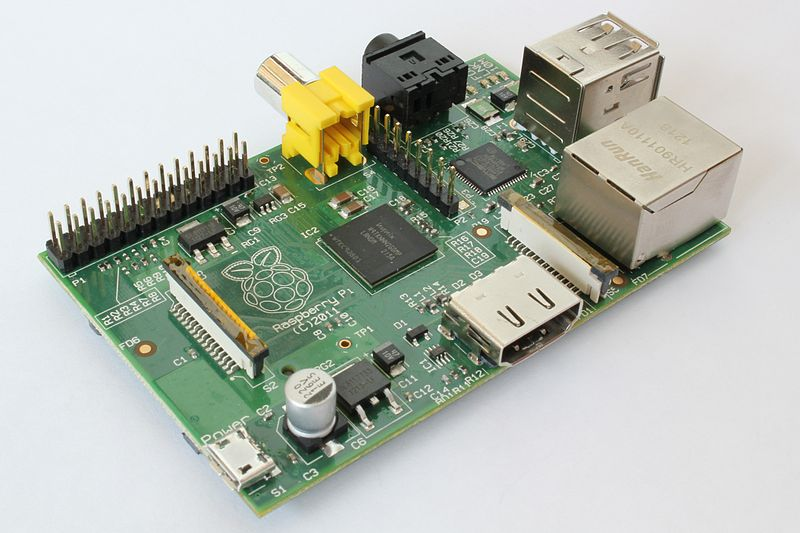
\includegraphics[width=9cm]{Raspi.jpg}
}
\begin{itemize}
\item 3,5-mm-Klinkenstecker (analog), HDMI (digital)
\item Kartenleser für SD (SDHC und SDXC)/MMC/SDIO
\item 10/100-MBit-Ethernet-Controller 
\item 5 V, 700 mA (3,5 Watt)
\item 5-V-Micro-USB-Anschluss (Micro-B), alternativ 4 x AA-Batterien
\end{itemize}

Für Test und Kontrollausgaben benutzen wir einen am HDMI-Ausgang angeschlossenen Monitor.

Für den Anschluss an einen Bildschirm benutzen den HDMI Ausgang.
Diesen benutzen wir für Kontrollausgaben und Tests.

Als Stromquelle steht ein Akkupack ......(Firma,Modell) zum Einsatz. 
Hierbei ist wichtig, dass der Raspberry mind. 700 mA, besser 1 A zur Stromversorgung bekommt. 
Bei niedrigerer Amperzahl arbeitet der PC oft nicht zuverlässig.

Ein schneller und großer RAM Speicher ist für unsere Zwecke wichtig, da viele Signale, teils sogar synchron, verarbEin 17-Zoll Monitor wird für die Bildschirmausgabe des Raspberry über HDMI zu DVI benutzteitet werden müssen.

Für die Datenübertragung über das Netz benutzen wir einen Standard 300Mbit/s Wlan-Stick.

Der Raspberry Pi arbeitet mit einer ARM-Prozessorarchitektur.
Diese Architektur wird gerne für embedded Systems, wie PDAs oder Router, eingesetzt.

Sie ist auch auf jedem Smartphone zu finden, da sie den Vorteil einer sehr geringen Leistungsaufnahme bietet. 

%Konfiguration von Linux???
Erwähnenswert ist die Architektur deshalb, weil wir im Laufe des Projektes Schwierigkeiten hatten, auf die wir später eingehen werden
Wir benutzen das auf Linux basierende Betriebssystem Raspbian.
Dabei handelt sich um ein für Raspberry Pi optimiertes open-source Debian-System.
Es enthält viele für die ARM-Architektur vorkompilierte Pakete (über 35.000), dazu auch Features wie etwa eine GUI.

Das System braucht 3GB Speicherbedarf unserer 16GB großen SD-Karte.
Der zusätzliche Speicherplatz wäre nötig, falls man vorhat, Log-Dateien und Ähnliches direkt auf dem Raspberry Pi zu speichern. 
In unserem Fall übernehmen das jedoch die leistungsstärkeren PC's über das ROS Netzwerk.

GPIO (General Purpose Input/Output) ist ein weiteres interessantes Feature des Raspberry Pi.
Es gibt uns die Möglichkeit, jegliche Hardware-Funktionalität anzusteuern.
Beispielsweise können LED-Leuchten oder der Start-Knopf der Kaffeemaschine damit über ROS gesteuert werden.
Wir konnten uns leider jedoch zeitlich bedingt nicht mehr mit dieser Thematik beschäftigen, es bietet aber Anreiz für noch mehr Ansätze und Umsetzungen mithilfe des Raspberry Pi und ROS.

\subsection{ROS}
%Zitate??
ROS ist kein eigentliches Betriebssystem im herkömmlichem Sinne, sondern eine Art strukturierte Kommunikationsschicht.
Die Ziele von ROS können zusammengefasst werden zu:
\begin{itemize}
\item Peer-to-peer (System mit vielen laufenden Prozessen auf verschiedenen Hosts)
\item Tool-based (microkernel Design bestehend aus vielen Komponenten, ähnlich zu Linux)
\item multi-lingual (unterstützt viele Computersprachen, z. B. Python, C++, etc.)
\item thin (Wiederverwendbarkeit von Code steht im Mittelpunkt)
\item open source and free (unter der BSD Lizenz)
\end{itemize}
Es ist das einzig existierende Framework, welches sich auf diese Kriterien spezialisiert.
Den Entwicklern von ROS ging es vor allem um die Vereinfachung, Software für eine hohe Zahl an verschiedenen Roboter zu schreiben.
%Zitat
ROS stellt dazu Bibliotheken und Werkzeuge, Hardware Abstraktion, Gerätetreiber, Bibliotheken, Visualisierungen, Nachrichtenvermittlung, Packetverwaltung und andere Komponenten zur Verfügung.

Im Nachfolgenden werden die wichtigsten ROS Core Komponenten kurz beschrieben.

{\bf Topic} Topics können als "named bus" gesehen werden, über welche Nodes Messages verteilen können. Es ähnelt dem Multicasting Prinzip. An Topics kann subscribed (zugehört) oder published (geredet) werden.

{\bf Node} Eine Node ist ein simples Programm, welches jede Funktionalität ermöglicht.  Sie kommunizieren direkt über oben genannte Topics.

{\bf Roscore} Der Roscore kann als Rückgrat des ROS Systems beschrieben werden. Es verwaltet die Registrierung der Nodes und Funktionen in einer Art lookup service für andere Nodes. Es bietet zusätzlich einen Parameter Server, in welchem im Laufenden Betrieb Variablen und Paramater gespeichert werden können und mit welchen gearbeitet werden kann.

{\bf Message} Eine Message kann als Sprache angesehen werden, in welcher Nodes kommunizieren. Es ist eine Struktur aus simplen Parametern.
Beispiel:
\begin{verbatim}
	# This represents a vector in free space. 
	float64 x
	float64 y
	float64 z
\end{verbatim}
Eigene Messages mit den uns bekannten Standardtypen wie int, bool, etc können leicht definiert werden.

{\bf Package} Software in ROS wird mithilfe von Packages verwaltet.
Sie enthalten Nodes, datasets, configuration files, etc.

{\bf Manifest} Sie enthält Meta Informationen über ein ROS Package, wie beispielsweise Abhängigkeiten oder Lizenzinformationen.

{\bf Launchfile} Ein Launchfile ist eine simple XML Datei, welche Informationen über die zu Beginn zu startenden Nodes mit entsprechenden Parametern enthält.
Dies bietet eine komfortablere Alternative, als jedes Node einzeln zu starten.
%Beispiel??
 
{\bf catkin} Catkin ist das seit Groovy in ROS verwendete Workspace-Verwaltungssystem.
Es ist in 4 Spaces unterteilt:
\begin{itemize}
\item Source Space
\item Build Space
\item Devel Space
\item Install Space
\end{itemize}
Catkin bietet uns eine komfortable Möglichkeit über cmake, ROS Packages zu compilieren, Tests an Ihnen durchzuführen und sie schließlich zu installieren.

\subsection{Volksbot}
\parbox{8cm}{
VolksBot ist ein Roboterbaukastensystem.
Mit Hilfe des Baukastens können sehr schnell und preiswert unterschiedlichste Varianten mobiler Roboter hergestellt werden.
Der Volksbot wurde an der Hochschule Weingarten für den RoboCup verwendet.
}\hfill
\parbox{5cm}{
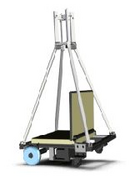
\includegraphics[width=5cm]{Volksbot.jpg}
%TODO Wir brauchen hier mehr Infos, wo wurde er verwendet, Besonderheiten<-- evtl nicht soo wichtig
%TODO Bild
}
\subsection{Smartphone}

Es wird ein auf Android basierendes Smartphone verwendet.
Wir benutzen auf dem Smartphone eine in einer Projekt-Arbeit entstandene App.
Sie bindet sich an einen ROS-Master (später näher erläutert) und übergibt die X und -Y Koordinaten relativ zu sich weiter.
Diese Werte können für die Steuerung des Motors verwendet werden, indem jeweils ein Wert an eine Radachse geliefert wird. Dieser Wert bildet die Geschwindigkeit des Rades ab.
Zur erleichterten Bedienung stellt uns die App eine GUI zur Verfügung. 

\section{Problem}

Viele der heutigen Roboter mit ROS-Systemen besitzen einen leistungsstarken und klobigen PC an Ihrer Seite.
Doch für viele Roboteranwendungen würde auch ein kleinerer, leistungschwächerer PC ausreichen.
Dadurch ergeben sich neue Vorteile.

\begin{itemize}
\item weniger Gewicht
\item weniger Kosten
\item Energieverbrauch sinkt $\rightarrow$ Akku hält länger
\item Die Größe des Roboters nimmt ab
\end{itemize}

In unserem Fall wird der Roboter Volksbot mit einem für diesen Zweck überdimensionierten Laptop gesteuert. Wir wollen dieses Problem beheben und uns die obigen Vorteile verschaffen, indem wir ROS auf einem Raspberry Pi laufen lassen.

\section{Verwandte Arbeiten}

Master-Thesis:
\begin{enumerate}

\item Robot Navigation in Unknown Environment Based on Combined 2D and 3D Information, Marc Götz, August 2013
\item Semi-Autonomous Grasping of Unknown Objects, Steffen Pfiffner, November 2013
\end{enumerate}

\section{Anforderungen}

Mit diesem Projekt haben wir das Ziel, ROS auf dem Pi zu testen und an einem gegebenen Roboter anzuwenden. Aus diesem Ziel, sowie den vorangegangenen Punkten, erschließen sich für uns folgende Anforderungen:
\vspace{0,4cm}
\begin{itemize}
\item Datenpakete über das ROS-Netzwerk verschicken
\item Beliebige Datentypen verarbeiten
\item Überprüfung von Log-Dateien, Kontrollausgaben etc..
\item Robuste und zuverlässige Kommunikation
\item Modulares und flexibles Netzwerk
\item Repositories sollen leicht in Projekte eingebunden werden

\vspace{0,6cm}

\item Roboter soll bei Steuerung in die richtige Richtungen fahren
\item Roboter soll sofort auf Anweisungen reagieren
\item Sensibilität der Steuerung sollte einstellbar sein
\item Steuerung über WLAN
\item ROS-Core des Raspberry beim Hochfahren automatisch starte
\item Leichte Bedienbarkeit des Roboters

\vspace{0,6cm}

\end{itemize}

{\bf optional}

\begin{itemize}
\item Streaming-Bild ruckelfrei verarbeiten
\item unkonvertiert Echtzeitübertragung
\item Ausgabe am externem Bildschirm
\end{itemize}


\section{Lösungsvorschläge}

{\bf Datenpakete über das Netzwerk verschicken:}\\
Es wird ein ROS-Master aufgesetzt. Dieser gilt als Knotenpunkt (vergleichbar mit einem Defaultgateway) und sorgt für die Kommunikationsmöglichkeit im ROS-Netzwerk.

{\bf Beliebige Datentypen verarbeiten:}\\
Die Verarbeitung von verschiedenen Datentypen ist durch msg und srv realisierbar
%TODO msg/srv näher erklären

{\bf Überprüfung Kontrollausgaben:}\\
Kontrollausgaben und ähnliches werden durch Horchen an Topics mithilfe von echo und durch Ausgabenbereiche im Quellcode durch das Netzwerk realisiert.
 
%Horchen an Topics mit echo + Ausgabe im Code mithilfe ROS-Stream Fkt.

{\bf Zuverlässige Kommunikation:}\\
Die Netzwerkstabilität und -zuverläsigkeit könnte durch Begrenzung der zeitgleichen Datenübertragung umgesetzt werden. Zusätzlich kann man eine Überprüfung der verschickten und erwarteten Datentypen einbinden.

%Verschickte und erwartete Datentypen müssen stimmen
%Richtige Konfiguration des Masters und Clients

{\bf Flexibles Netzwerk, Repositoryeinbindung:}\\
Ein Modulares und flexibles Netzwerk, sowie das einfache Einbinden von Repositories ist durch ROS in Kombination mit Catkin gegeben. Diese Features müssen allerding zuvor aktiviert werden.
%TODO umschreiben!

\vspace {0,6cm}

%Roboter soll bei Steuerung in die richtige Richtungen fahren
{\bf Steuerung eines Roboters:}\\
Die Reaktionszeit und Steuerung wird durch zuverlässige und leistungstarke Hardware, sowie durch einen effizient geschriebenen Code bestimmt. In diesem Fall können wir die Hardware (mit ausßnahme des Pi) aufrüsten. Der Code lässt sich gar nicht oder nur mühsam verändern und austauschen.
%abhängig vom richtigen Code der Motorsteuerung

%abhängig von Raspberry Pi Hardware und effizientem Code und
%guter Hardware
{\bf ROS-Core automatisch starte:}\\
Um bequem mit dem Raspberry arbeiten zu können, ohne jedes mal den ROS-Core starten zu müssen, muss dieser in den Bootvorgang des Raspbian eingebunden werden.

{\bf Leichte Bedienbarkeit:}\\
Diesen Punkt wollen wir mit einer Smartphone App realisieren. Der Roboter soll dabei auf das Schwenken des Smartphons reagieren und seine Geschwindigkeit/Richtung entsprechend anpassen.
%gegeben durch gute Smartphone App

\vspace{0,6cm}

{\bf Videoübertragung:}\\
Ein sauberes und störungsfreies Übertragungsbild hängt hauptsächlich von der Hardware des Raspberry Pi, aber auch von der Codierung ab. Der Stream soll durch  Umleiten des Bildes über das Netzwerk an einen PC-Monitor realisiert werden. Falls dabei Probleme auftreten sollten, können wir versuchen die Codierung zu bearbeiten oder leistungsverstärkende Hardware an den Pi anschließen.

%abhängig von Raspberry Pi Hardware und Übertragungs-Codierung

%abhängig vom Codex Hardware Komponenten

%nötige Hardware und Netzwerk legen

\section{Bewertung der Lösungen}

Bis jetzt sind unsere Lösungsansätze realativ erfolgreich gewesen. Es könnten jedoch Probleme bei der Steuerung des Roboters über das WLAN-Netzwerk entstehen. Der Grund dafür ist die zusätzliche Datenmenge, die verarbeitet werden muss.

\section{Implementation}

\subsection{Raspbian}

Zuerst wird das Betriebssystem Raspbian auf dem Pi aufgesetzt.
Hierzu gibt es 2 mögliche Vorgehensweisen:
\begin{enumerate}
\item Installation mit NOOBS
\item Flashen der SD-Karte (Linux mittels dd)
\end{enumerate}

Wir haben uns für die 2. Methode entschieden, da NOOBS 6 verschiedene Images anbietet, doch wird in diesem Fall nur Raspbian benötigt.
Zudem erfordert die 2. Vorgehensweise mehr Arbeit mit dem Linux Betriebssystem, was in dieser Vorlesung nur vorteilhaft sein kann.
Die genauen Installationsschritte entnehmen Sie bitte der Quelle (raspbian...) unter dem Unterpunkt Using the Linux command line. \\
Um mögliche Fehlerquellen schon beim Herunterladen der Image Datei zu vermeiden, wird empfohlen, wie in der Anleitung beschrieben die sha1sum zu vergleichen.
%\begin{enumerate}
%\item Mit df -h herausfinden, welchen Namen die SD-Karte trägt (z. B. sdb)
%\item mit dd bs=4M if=~/2012-12-16-wheezy-raspbian.img of=/dev/sdd Image %auf SD-Karte schreiben
%\end{enumerate}

Nun muss nur noch die SD-Karte in den Raspberry eingesteckt werden. Falls eine grüne Leuchte am Raspberry blinkt oder eine Bildschirmausgabe an einem Monitor erscheint, ist dieser Schritt gelungen.

\subsection{ROS aufsetzen}
Willow Garage stellt seit der Entstehung von ROS mehrerere Distributionen zur Verfügung.
Für den Raspian ist die momentan zweitaktuellste Distribution Groovy zu empfehlen. 
Die aktuelle Version Hydro wird noch nicht unterstützt. \\
Es gibt 2 sinnvolle Wege, ROS Groovy auf dem Raspbian System aufzusetzen.
%Vorteile, Nachteile
\begin{enumerate}
\item Source packages des ROS-Kerns kompilieren
\item binary packages für die ARM-Architektur installieren
\end{enumerate}

Da die Installation und das Kompilieren von Source zwar sehr lehrreich, doch auch relativ zeitaufwendig ist, benutzen wir die vorhandenen binary packages für ARM. 
Hierzu einfach nach dieser Anleitung vorgehen (Quelle..) \\
Leider werden dadurch nur die grundlegendsten Packages von ROS unterstützt.
Da ein großer Vorteil von ROS die Modularität ist, können leicht benötigte packages über catkin nachinstalliert werden.
Dazu weiter unten die Vorgehensweise erklärt am Beispiel des packages zur Steuerung des Roboters.\\
\\
%welche, näher erläutern, sourcen
ROS integriert sich sehr gut in die Shell des Linux Systems ein.
Unterstützt werden mehrere Shell-Typen. In diesem Projekt wird die Bourne Again Shell verwendet.
ROS bietet für seine Systemumgebung Äquivalente zu den wichtigsten Shell Befehlen, beispielsweise roscd für cd oder rosls für ls. \\
Dadurch ergibt sich der Vorteil, nicht den vollständigen Pfad zu einem ROS package oder Verzeichnis eingeben zu müssen. Beispielsweise ist es möglich sofort in ein ROS Verzeichnis mit roscd zu wechseln, ohne den vollständigen Pfad mittels cd eingeben zu müssen. \\
Damit man auf die ROS typischen Shell Befehle Zugriff hat, muss zuerst gesourced werden.

 \begin{lstlisting}
 source /opt/ros/groovy/setup.bash
 \end{lstlisting}

Der Source Befehl bewirkt, dass die Pfade zu den ROS Verzeichnissen dem Linux System bekannt gemacht werden.
%TODO hier vllt. Bild des Inhaltes von ROS
%Shell Bilder, Bsp. von Kommandos
%TODO in .bashrc eintragen!!

Es empfiehlt sich, sich mit den typischen ROS Befehlen etwas vertraut zu machen. (Quelle... Tutorials) \\
Mit diesen Einstellungen sollte es kein Problem mehr sein, ein Netzwerk zwischen Systemen aufzusetzen.
\subsection{Netzwerk aufsetzen}
%Vorrausetzungen für das ROS Netzwerk
Damit ein Netzwerk aufgesetzt werden kann, muss ein Linuxsystem zum Master werden.
%Zu diesem Zweck gehen Sie bitte nach diesem Tutorial vor (Quelle %http://wiki.ros.org/ROS/Tutorials/MultipleMachines)
Im Grunde ist es wichtig, in allen Systemen des Netzwerks in export die IP-Adresse und die Port-Nummer (Standard: 11311) des Systems anzugeben, welches als Master dienen soll.
Eine der Möglichkeiten sich die IP-Adresse des Systems anzeigen zu lassen ist der Shell Befehl ifconfig.
%TODO %Bild von ifconfig einfügen + Highlighting der IP
Die IP lässt sich leicht aus den Informationen herauslesen.

{\bf ROS Workspace anlegen:}

Für ROS sollte noch ein Workspace mit catkin erzeugt werden.
Quelle: http://wiki.ros.org/ROS/Tutorials/InstallingandConfiguringROSEnvironment
4. Create a ROS Workspace
Auch das Sourcen des Workspace sollte am besten in die .bashrc, wie oben gezeigt, aufgenommen werden. \\
Es noch zusätzlich ein Beispiel package erzeugt, welches später zum Testen des Netzwerks erforderlich ist.
Dazu in das Source Verzeichnis des catkin Workspace wechseln

 \begin{lstlisting}
 cd ~/catkin_ws/src
 \end{lstlisting}

und ein package erzeugen. 

 \begin{lstlisting}
 catkin_create_pkg beginner_tutorials
 std_msgs rospy roscpp
 \end{lstlisting}

Das package sollte noch compiliert werden.
Erneut in  das catkin Workspace wechseln

 \begin{lstlisting}
 cd ~/catkin_ws
 \end{lstlisting}

und  
 
 \begin{lstlisting}
 catkin_make
 \end{lstlisting}
 
ausführen.
%Für uns ist der Befehl roscore wichtig.
%Wir setzen in unserer exports Datei die ROS!MASTER!URI IP-Adresse auf die %des Raspberry Pi und dazu den Standardport 11311.
%Dies macht den Raspberry zum Master Knotenpunkt, nun können andere Linux-%Systeme mit ROS über diesen kommunizieren.
%Sie müssen zusätzlich in der exports die ROS!MASTER!URI IP-Adresse des %Raspberry angeben.
\subsection{Testen des Netzwerks}

Um das bestehende Netzwerk zu testen, können Datenpakete zwischen den Systemen verschickt werden.
Zuerst sollte der Master ansprechbar sein.
Hierfür wird der Kern von ROS mit dem Shell Befehl 

 \begin{lstlisting}
 roscore
 \end{lstlisting}

gestartet. \\
%TODO Bild der Ausgabe des Kerns mit Highlighting der IP URI
Falls bei Eingabe des Befehls

 \begin{lstlisting}
 rosnode list
 \end{lstlisting}

als Antwort mindestens ein Node (/rosout) erscheint, läuft der Kern ordnungsgemäß. \\
Um nun einfache Testausgaben zwischen Systemen zu schicken, werden zwei ROS Nodes und ein Topic zur Kommunikation eingerichtet.
Auf dem ROS Master wird ein listener Node (Subscriber) gestartet, der Quellcode befindet sich unter 1.1.1 The Code. \\
Auf einem anderen ROS System wird ein talker Node (Publisher) gestartet, der Quellcode befindet sich unter 1.2.1 The Code. \\
%http://wiki.ros.org/ROS/Tutorials/WritingPublisherSubscriber%28python%29
Es kann auch der talker anstatt des listeners auf dem Master ausgeführt werden.
Es sollte nicht vergessen werden, die Quelldateien mittels

 \begin{lstlisting}
 chmod +x Dateiname.py
 \end{lstlisting}

ausführbar zu machen. \\
{\bf Alternative:}rqt C++ Code
%http://wiki.ros.org/ROS/Tutorials/WritingPublisherSubscriber%28c%2B%2B%29

Die Nodes mit dem Befehl 

 \begin{lstlisting}
 rosrun beginner_tutorials Dateiname.py
 \end{lstlisting}
 
starten.
Im Shell Fenster des Listener Nodes sollte nun die Ausgabe des Talker Nodes erscheinen.

%Bild einfügen
Falls dies nicht passiert, sollte die obige Anleitung noch einmal genau befolgt werden und zusätzlich das Netzwerk auf Fehler überprüft werden.
%http://wiki.ros.org/ROS/NetworkSetup

%TODO Auf dem Raspberry nicht möglich?=???!!!
Die Nodes und Topics können zum besseren Verständnis visualisiert werden.
Zuerst muss das rqt package installiert werden.

 \begin{lstlisting}
 sudo get-apt install ros-groovy-rqt
 \end{lstlisting}

Mit 

 \begin{lstlisting}
 rqt_graph 
 \end{lstlisting}

wird das Verhältnis der Nodes visualisiert.

%TODO evtl bild einfügen?

%Hierzu schicken wir mithilfe der App eine Message, welche die X und Y %Koordinaten enthält.

%Wir geben in der App die IP des Masters (Pi) an. Das Handy fungiert nun %als ROS Node und versendet (publish) diese Messages über einen Topic, an %welchem der Pi horcht (subscribe).

%Raspberry Pi kann nun mithilfe des ROS Befehls

%	rostopic echo ''Topicbezeichnung''
	
%aus diesem Topic alle Daten auslesen und ausgeben.
%Bilder der Testdaten
%Da die Koordinaten mit denen auf dem Handy übereinstimmen, ist der %Netzwerktest erfoglreich.

%kurze Info zu Services und Massages, hier wird nicht näher darauf eingegangen!!
%Link zu einem Tutorial bei Interesse
\subsection{Steuerung des Volksbot}

Für die Ansteuerung des Motorcontrollers des Volksbot benutzen wir ein in einer Projekt-Arbeit entstandenes ROS Package.
<<<<<<< HEAD
Nach einiger Konfiguration konnten wir dieses Package mithilfe catkin!make kompilieren und in unser Projekt integrieren.
Über eine roslaunch Datei wurden die nötigen Nodes und Topics des Packages gestartet.

Die Netzwerk-Funktionalität ist nach den obigen Tests gegeben.
Die Rohdaten des Smartphone-Sensors werden durch das ROS Steuerungspaket entsprechend verändert und über den Raspberry an den Volksbot gesendet.
Der Raspberry wird mithilfe eines USB zu VGA Adapters an den Volksbot angeschlossen. Dieser wird per USB an den Raspberry Pi und per VGA an das Steuerungsmodul des Roboters angeschlossen.


%TODO Konfiguration Motorsteuerung-Paket und Compilieren


%Kontrollausgaben:
%\begin{itemize}

%\item Horchen am ROS-Topic

%\subitem rostopic echo ''Topicbezeichnung''

%\item  

%\end{itemize}

%TODO Netzwerkkomponenten zusammen arbeiten lassen (Hard/-Software)


%TODO Wlan -> Teilproblem


%TODO Kamera -> Teilproblem Zeit


\section{Fazit}
\subsection{Zusammenfassung}

Sehr gut ist der Askept, dass man das Thema frei wählen konnte. Dadurch steigt das Interesse und die Motivation an der Arbeit. Durch die hohen Anforderungen und den knappen Zeitraum ist es aber auch sehr Anspruchsvoll und Arbeitsintensiv. 

%hohe Anforderungen für knappen Zeitraum
%interessantes, anspruchsvolles Projekt
%viel über Linux und Ros gelernt
%Hardware- und Netzwerkkonfiguration interessant

\subsection{Ausblick}

In Zukunft kann der Raspberry Pi durch die Tatsache, dass wir ROS benutzt haben, vielseitig im Robotiklabor verwendet werden. Zum Beispiel bei Projekten, die wenig Spielraum bei Größe und Energieverbrauch zulassen.
Durch die Tatsache, dass ROS immer mehr an Beliebtheit gewinnt, nimmt auch die Anzahl an binary-packages und Ausarbeitungen zu. Dies eröffnet wiederum mehr Einsatzmöglichkeiten.
Zum Beispiel kann man nicht nur Roboter, sondern durch das GPIO-Interface auch viele andere Hardwarekomponenten(wie die Bedienoberfläche einer Kaffeemaschine, Lichtschalter, etc.) steuern.  

%Benutzung des Pi's als Hardware Nodes Lab
%Benutzung des Pi's für kleine Roboterprojekte Lab
%Immer mehr binary packages für ROS Pi verfügbar -> mehr Möglichkeiten
%z.B.: GPIO Interface -> Knöpfe Kaffemaschine, Relays, alle möglichen Signale
%auf Hardwareebene

\subsection{Eigene Leistung}

Durch unser Projekt wird der Laptop am ''Volksbot'' durch einen viel kleineren und leichteren Raspberry Pi ersetzt. Außerdem eröffnet sich uns die Möglichkeit, den Pi als Hardware-Node zu benutzen oder anderweitig einzusetzten.

\section{Quellen}
\begin{verbatim}

http://de.wikipedia.org/wiki/Raspberry_Pi
http://www.amazon.de/Raspberry-Pi-RBCA000-Mainboard-1176JZF-S/dp/B008PT4GGC
http://www.raspbian.org/
http://www.softwareok.de/?seite=faq-System-Allgemein&faq=13
http://de.wikipedia.org/wiki/ARM-Architektur
http://www.rn-wissen.de/index.php/Raspberry_PI:_GPIO
http://www.raspberrypi.org/faqs <- bild Rasp
http://www.euron.org/maps/germany <- bild Volksbot

\end{verbatim}
%TODO überall quellen angeben
\end{document}
